\chapter{General-Purpose Computing on Graphics Processing Units}
General-Purpose computing on graphics processing unit (GPGPU) is the use of compute performance of graphics processing unit (GPU) for acceleration data-intensive or compute-intensive tasks.\\
These cards was originally designed for solving graphical tasks which require many vector or matrix computations on floating-point numbers so their architecture contains many simple cores for simple mathematical computations. This is their main advantage in comparison with ordinary CPU - they have ten times, a hundred times but lately thousand times more cores, so if the task could be vectorized, it could be accelerated up to hundred times on GPU in comparison to serial CPU version.\\
At the beginning, GPUs support only computation of vectors or matrices, usually two, three or four dimensional because of their origin, so general purpose computation had to be reformulated to this graphical principles supported by major graphics APIs like DirectX or OpenGL. This transformation was hard and many algorithms could not be transfered to graphical problems and could not be parallelized on GPUs.\\
This problem disappears later with the arrival of specialized frameworks for utilizing GPUs for general purpose programming. These frameworks allows to programmer to ignore limitations of graphics environment and make general computations easily.\\
Nowadays there exist two major frameworks for GPGPU - CUDA and OpenCL (open computing language). The main advantage of CUDA over OpenCL and other solutions is a direct link to the hardware, which is not the case of OpenCL and others. This is because CUDA is developed by Nvidia and only for Nvidia graphics cards so it could use concrete hardware specific properties. Compared to that, OpenCL by Khronos group is a universal, vendor independent framework for parallel computations supporting a large range of hardware divergent devices - it can be run on many CPUs and GPUs including Nvidia. This wide support of devices is a problem for high performance computing because OpenCL could not use every property of concrete architecture and hardware simply because there is nothing like concrete architecture. In the opposite CUDA is designed only for cards by Nvidia so it benefits from a small range of supported devices. In this work, we decided to use CUDA for one of the best performances among other frameworks and because we will not take main OpenCL advantage, the portability.\\
Other advantage of CUDA is that the device code and host code are written together and that they are both compiled in compile time in difference to OpenCL which compile device code at runtime.

\section{CUDA workflow}
When we want to launch CUDA program, first think what we must do in host code is detect. When desired device is selected, we could start with copying data from host to device. This action is asynchronous so we must synchronize execution of host code and memory transfer. When data transfer is done, we could launch device code called \textbf{kernel}. Kernel is same as normal C function but defined with special declaration and it can use special device functions. The set of function supported by concrete device is called \textbf{Compute Capability} (CC). This CC describes the device characteristics and a set of instructions that are supported. CC is tightly coupled with architecture (CC 1.x was supported by Tesla architecture, CC 2.x by Fermi, 3.x by Kepler, 5.x by Maxwell).\\
Kernel is launched from host code same as normal function but it runs asynchronously. This function is executed $N$ times in parallel by different CUDA threads. Number of threads is specified at function call. Threads are arranged in one, two or three dimensional space so it could easily compute with vectors, matrices or volumes. This bunch of threads is called \textbf{block}. The number of threads in block is limited because all threads in block must reside on the same core and must share the memory resources of appropriate core so on current GPUs, maximum number of threads is 1024.\\
The total number of threads is multiplied by number of blocks. Blocks could be also arranged in one, two or three dimensional space. Only limitation is that each block must be equally shaped so usually the number of thread blocks is determined by size of data being processed or by total number of cores. So total number of threads which executed single Kernel is number of threads times number of blocks as specified on~\ref{fig:cudagridthreadblock}. Kernel is also called asynchronously so when kernel is executing, host could for example start another memory transfer or doing another work. After synchronizing with device, we need usually transfer results from the device back to host which is again asynchronous call and must be synchronized.

\begin{figure}[h]
  \centering
  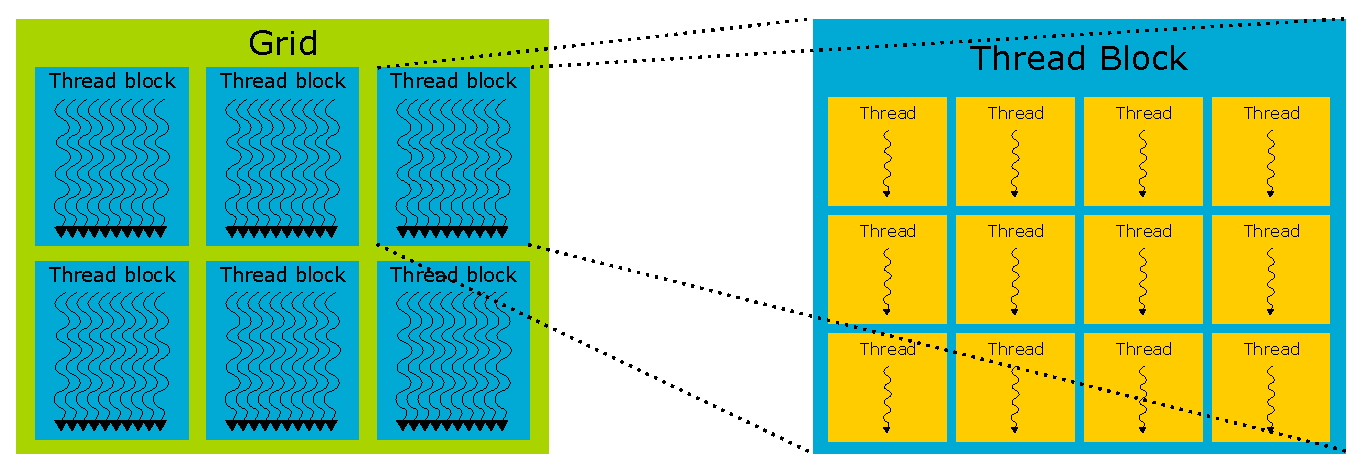
\includegraphics[width=1\linewidth]{img/CUDAthreadGridBlock.eps}
  \caption{2-dimensional Grid of 2-dimensional Thread Blocks}
  \label{fig:cudagridthreadblock}
\end{figure}

\section{GPU and CPU comparison} \label{ssec:gpucpucomparison}
Main difference between CPU and GPU is in their specialization. Instead of general purpose of CPUs, GPUs are specialized on graphics, which is computes with vectors and matrices, so GPU architecture is targeted for parallel vector work. The single cores are significantly different too because CPU core usually works on higher frequency (thousands of MHz)and supports many instructions in comparison to GPU core which works on lower frequencies (hundreds of Mhz) and supports only special set of instructions. Problem was the special designation of GPUs but after GPGPU was introduced, problem with GPU specialization was solved by special frameworks and GPUs began to compete with processors. Main differences between CPUs and GPUs are:
\begin{description}
\item[Number of cores] CPU has only few physical cores~\autoref{fig:cpuarchitecture}. Common CPUs have around 8 logical cores, server CPUs could have more, but usually it is between 32 and 64 cores on chip. Compared two that, modern GPUs have around thousand CUDA cores~\autoref{fig:gpuarchitecture}, the best models have around 2048 CUDA cores, so they have great potential for parallel tasks.
\item[Core architecture] GPU cores are specialized for numeric computations, not for general tasks as CPU cores, but because of their specialization, they compute numeric tasks really fast. CPU advantage is frequency, usually, CPU core is ten times faster than GPU core. This is because it is really hard to take away heat generated by thousands of cores placed on single chip so these cores must work on much lower frequency.
\item[Threads] Approach to threads is also different. CPU can process threads from different tasks at one time, which is called Simultaneous Multithreading (SMT), GPU uses Simple Instruction Multiple Thread (SIMT) pattern, which means that multiple threads run on same code and based on their identification, they could work on different branches or access different data.
\item[Memory] CPUs use big cache memory for hide latency of memory access so when thread is switched to different core, there is problem witch locally cached data, which are useless on original core and must be re-cached on new core. GPU has only small caches, because most of memory is on device, so context switch can be performed really fast.
\end{description}

\begin{figure}[h]
\centering
\begin{subfigure}{.49\textwidth}
  \centering
  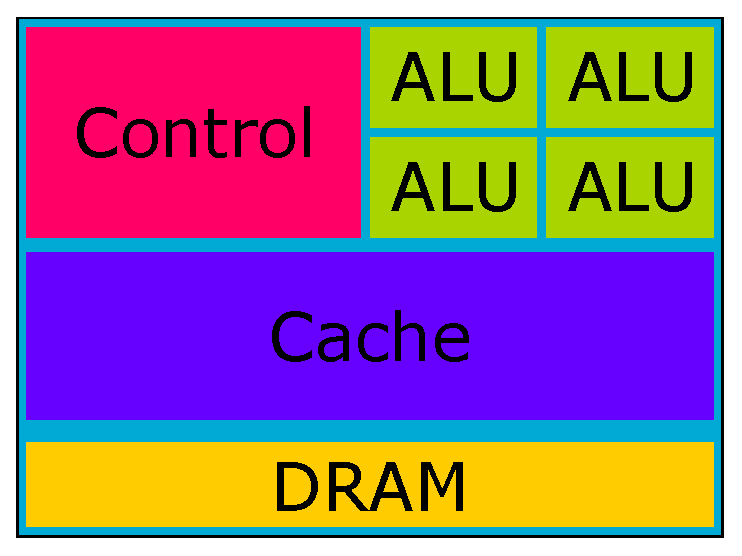
\includegraphics[width=1\linewidth]{img/CPUarchitecture.eps}
  \caption{CPU architecture}
  \label{fig:cpuarchitecture}
\end{subfigure}
\begin{subfigure}{.49\textwidth}
  \centering
  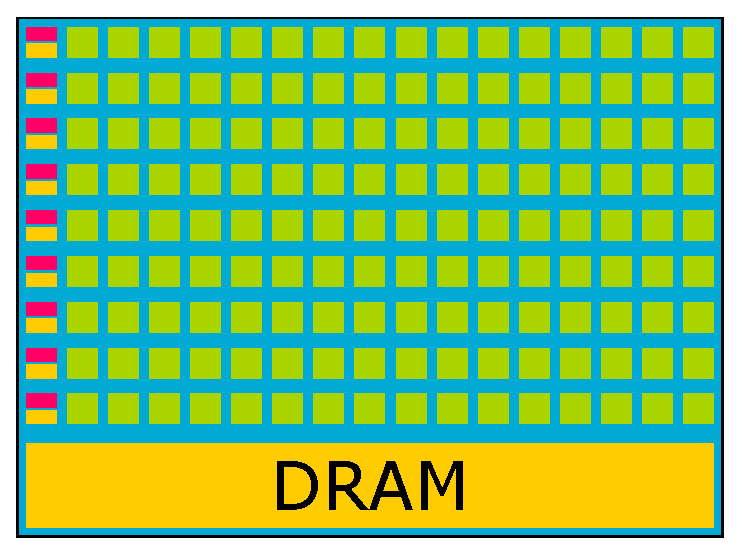
\includegraphics[width=1\linewidth]{img/GPUarchitecture.eps}
  \caption{GPU architecture (Fermi)}
  \label{fig:gpuarchitecture}
\end{subfigure}
\caption{CPU and GPU architecture comparison (same colors of boxes in GPU means same units)}
\end{figure}

%\begin{table}
%\begin{tabular}{|l|l|l|}
%\cline{1-2}
%NIC & CPU & GPU \\ \cline{1-2}
%# cores & Few cores per chip & Many cores per chip \\ \cline{1-2}
%Specialization & General purpose cores & Cores psecialized for numeric computations \\ \cline{1-2}
%Threads approach & Processing different threads & SIMT thread processing \\ \cline{1-2}
%Memory access & Huge caches to reduce memory latency & Huge amount of threads and fast context switch \\ \cline{1-2}
%\end{tabular}
%\end{table}
\section[Compute Unified Device Architecture]{Compute Unified Device Architecture\\ (CUDA)}
CUDA is parallel computing platform developed by Nvidia including software architecture integrated on Nvidia graphics cards. There exist more solutions than this one from Nvidia, but CUDA is one of the best for high performance computing. \\
CUDA use Simple Instruction Multiple Thread (SIMT) model, which is more flexible than Simple Instruction Multiple Data (SIMD) model, but generally, it has less performance. Both models approaching parallelism by broadcasting same instruction to multiple execution units, so only one instruction fetch/decode unit is needed by many execution units. Difference is that SIMT also have multiple register sets and addresses. Main difference is that SIMD processes short vectors in parallel and always all threads do the same work. For example, when we need sum two vectors, SIMD must iterate through vectors and in one step, it can only process as many elements as a computing units count is. On CUDA with SIMT model, we launch as many threads as size of vector and each thread can store values in own register.\\

\begin{figure}[h]
\centering
%\begin{subfigure}{0.49\textwidth}
%  \centering
%  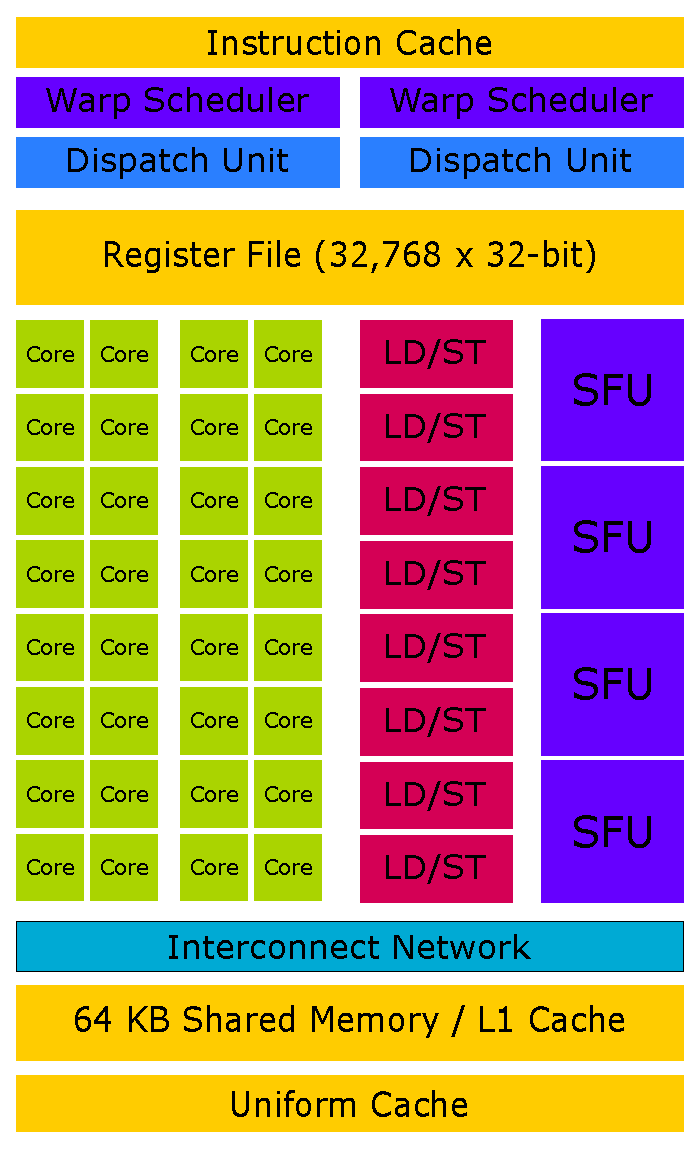
\includegraphics[width=0.8\linewidth]{img/SMPArchitecture.eps}
%  \caption{SMP architecture (Fermi)}
%  \label{fig:smparchitecture}
%\end{subfigure}
%\begin{subfigure}{0.6\textwidth}
  %\centering
  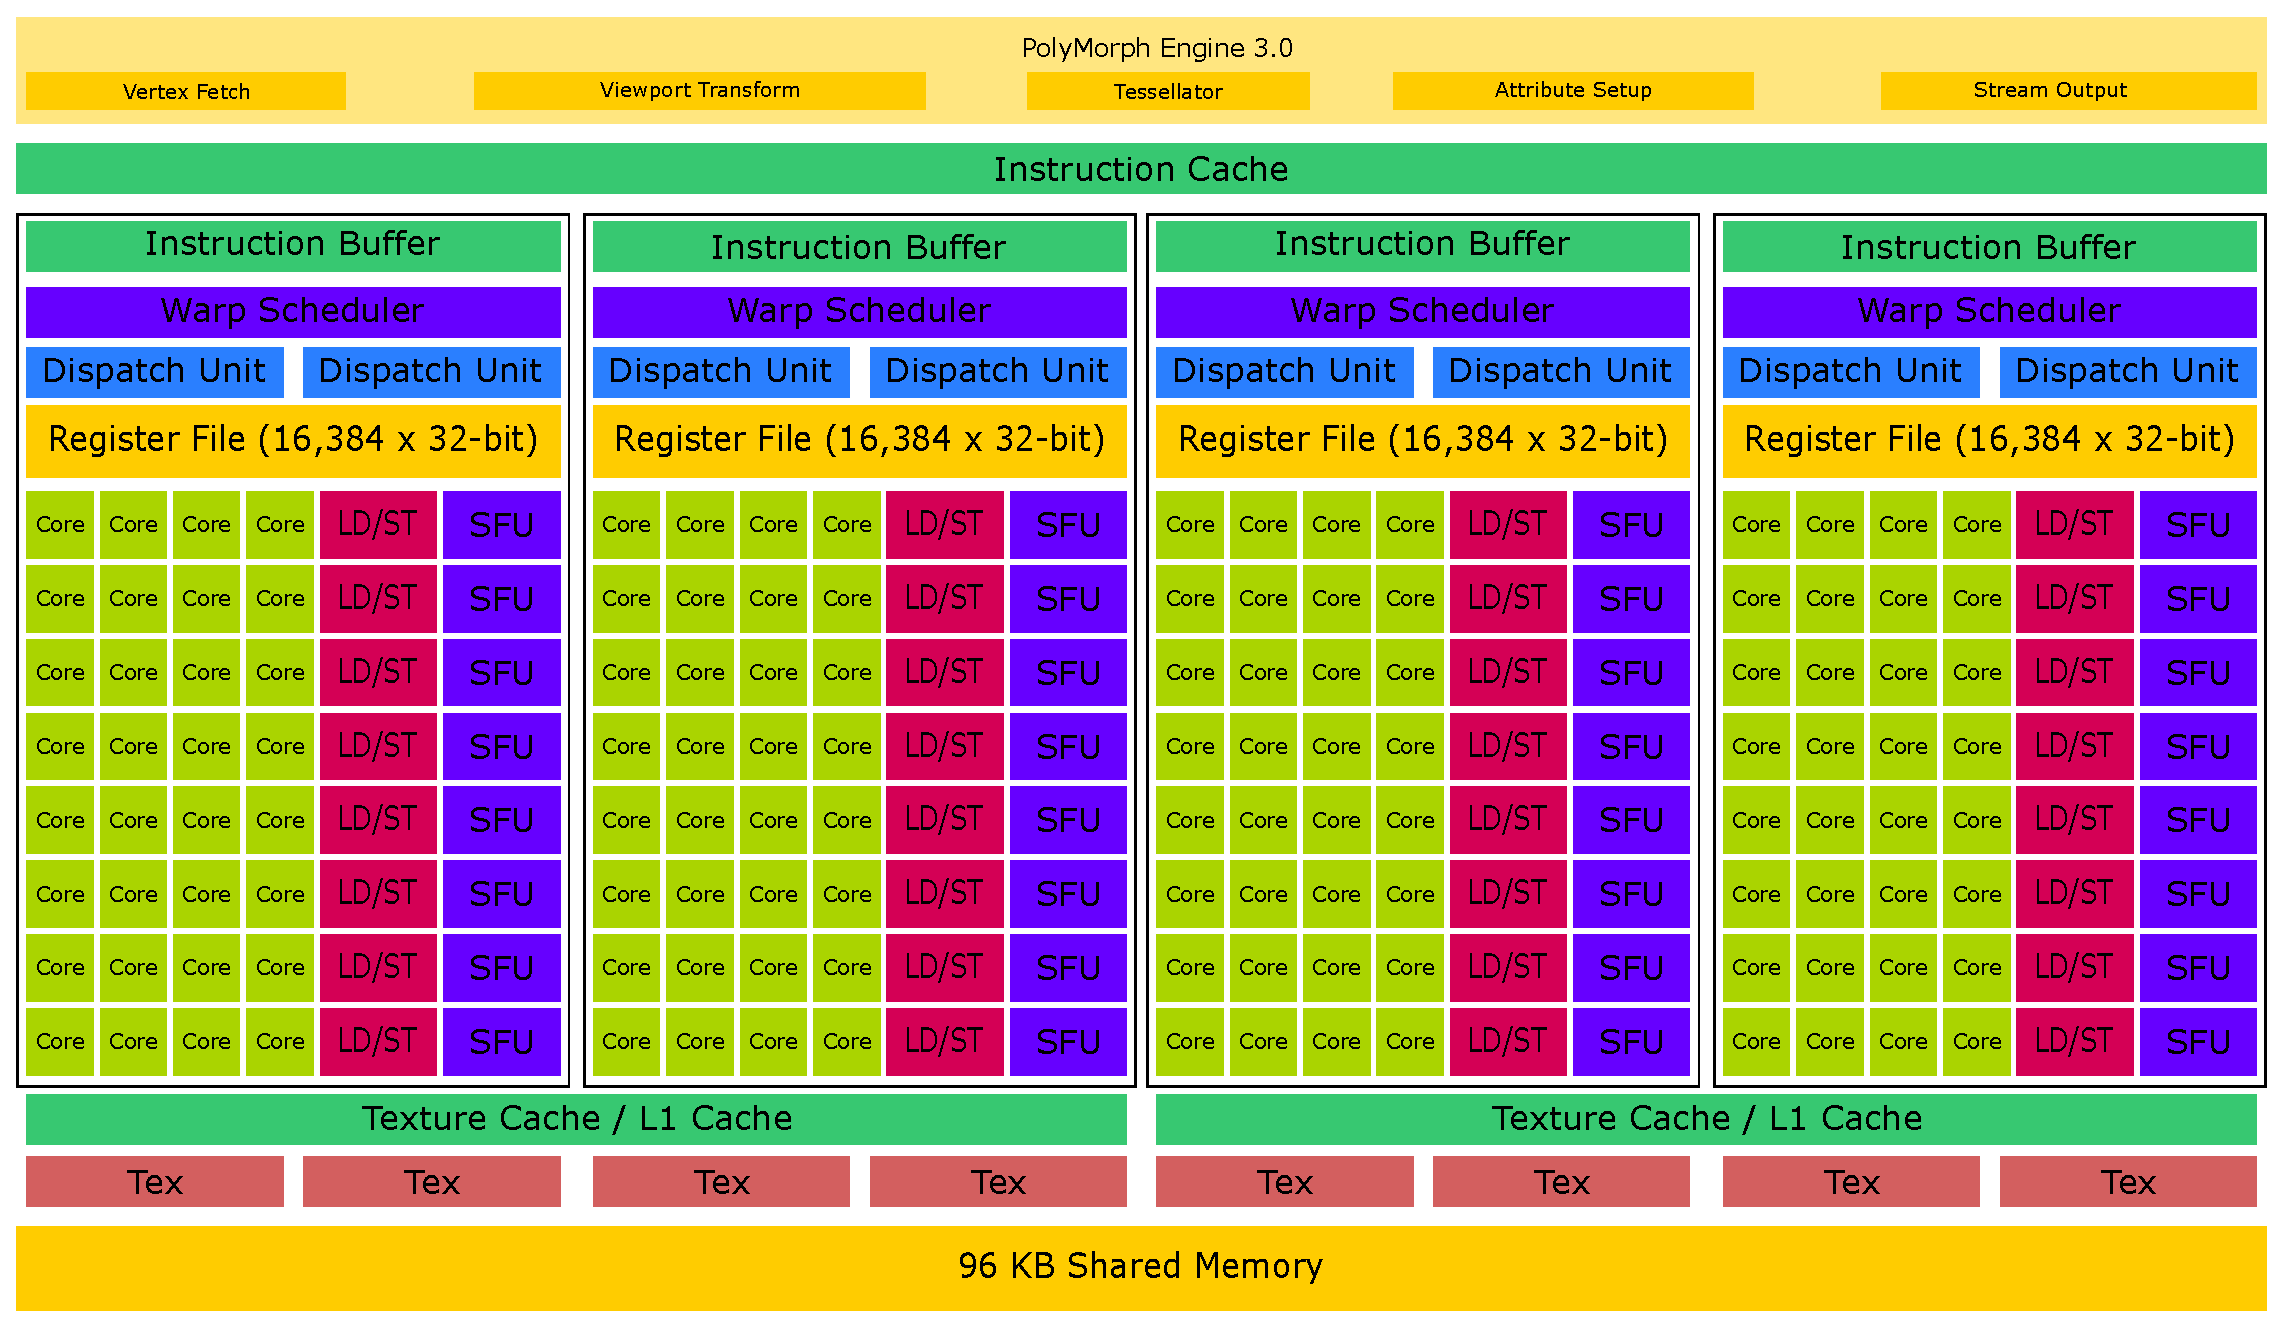
\includegraphics[width=1\linewidth]{img/SMMArchitecture.eps}
  \caption{SMM architecture (Maxwell)}
  \label{fig:smmarchitecture}
%\end{subfigure}
%\vspace*{0.1cm} 
%\begin{subfigure}{0.6\textwidth}
%  \centering
%  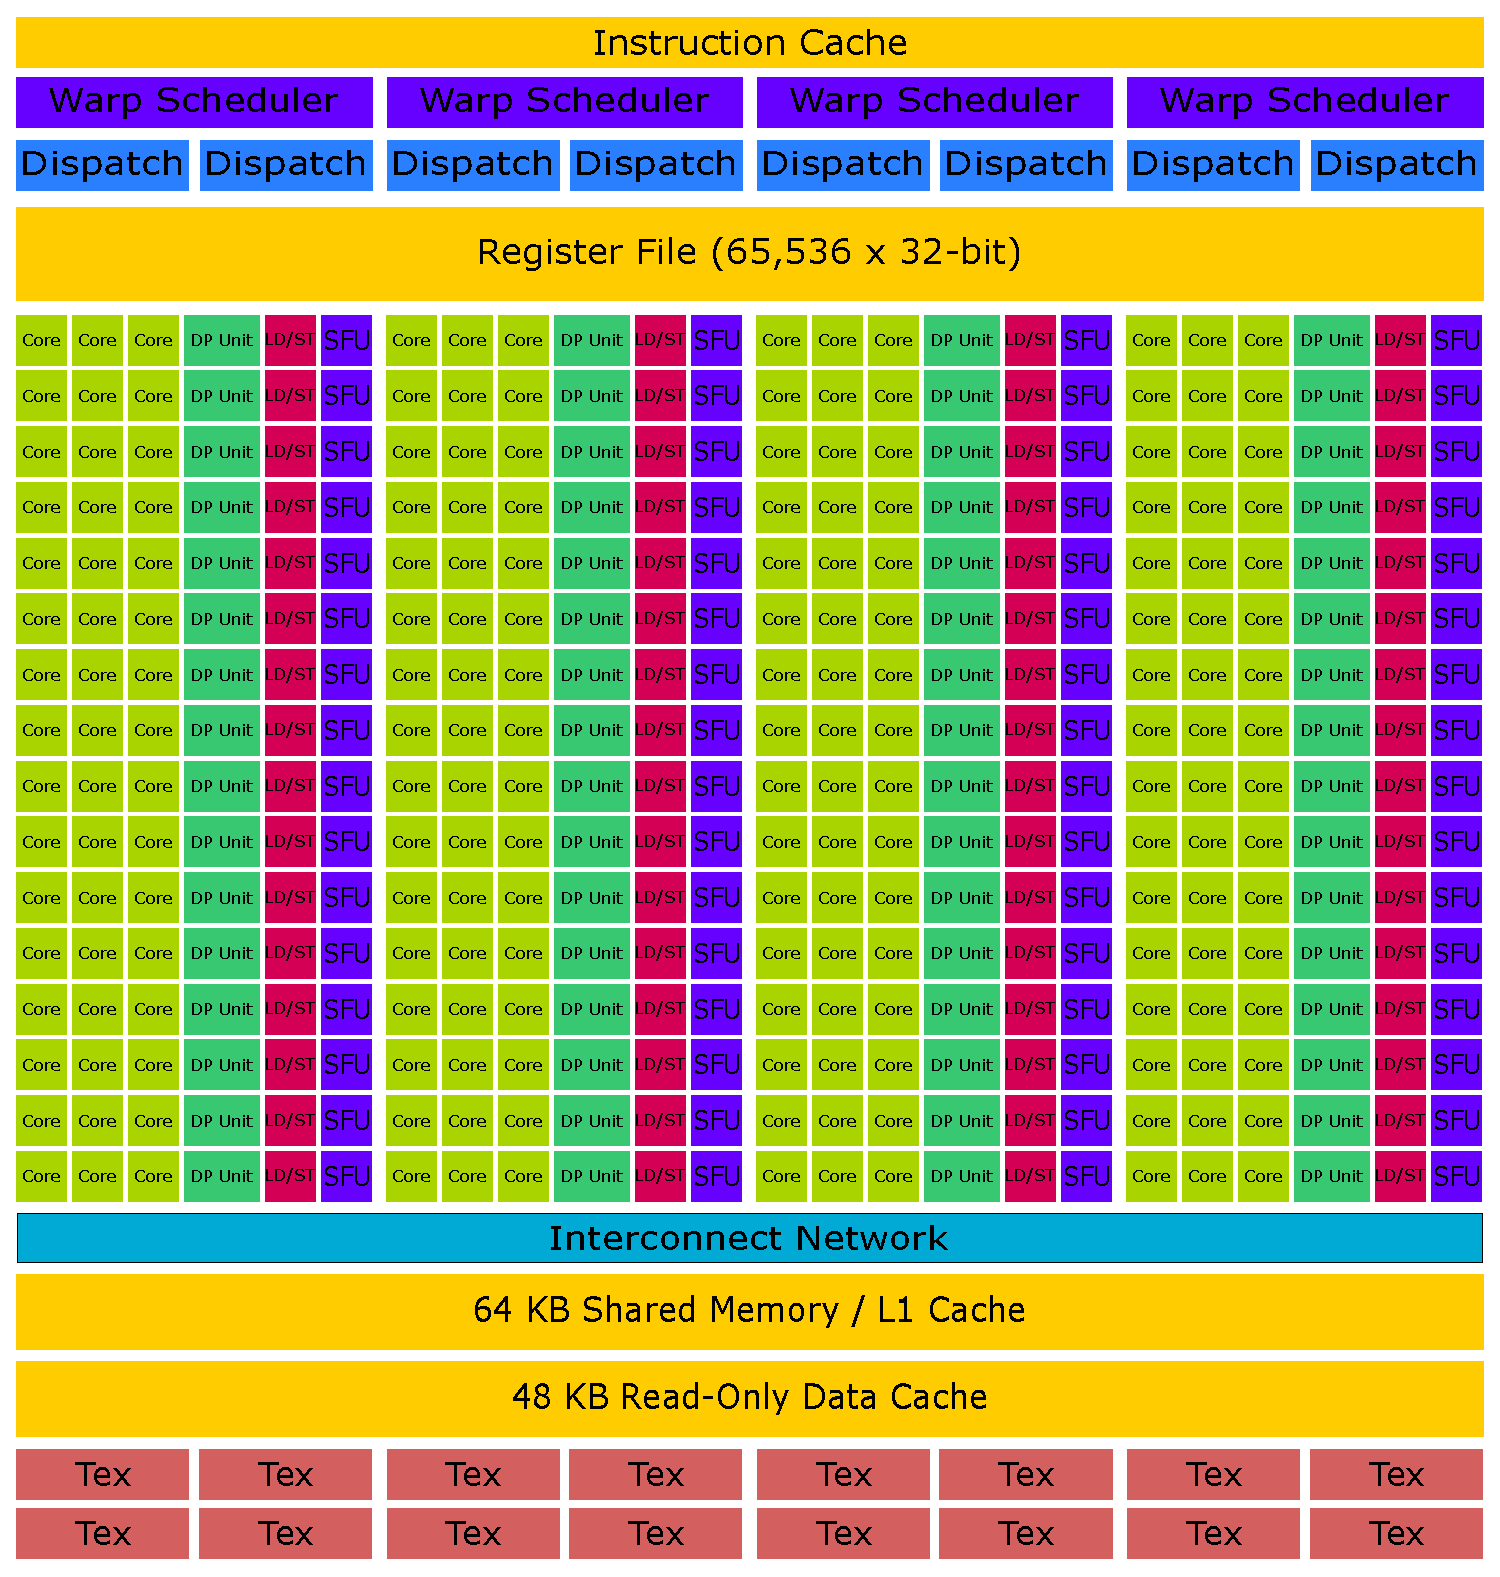
\includegraphics[width=0.9\linewidth]{img/SMXArchitecture.eps}
%  \caption{SMX architecture (Kepler)}
%  \label{fig:smxarchitecture}
%\end{subfigure}
\end{figure}

CUDA architecture contains larger processors called \textbf{Streaming Multiprocessor (SM)}. The oldest is \textbf{SMP} - Fermi, \textbf{SMX} - Kepler and the newest \textbf{SMM} - Maxwell~\autoref{fig:smmarchitecture}. Each SMP contains processor cores with registers (from 32 on Fermi architecture, 128 on Maxwell architecture and 192 on Kepler architecture), load/store units (LD/ST), Special Function Units (SFUs), shared instruction cache, shared memory and data caches. LD/ST and SFUs are shared by groups of cores, size of group depends on architecture.

\begin{figure}[h]
  \centering
  \includegraphics[width=0.8\linewidth]{img/CUDAmemoryHierarchy.eps}
  \caption{CUDA Execution model}
  \label{fig:cudamemhierarchy}
\end{figure}

Because number of cores is significantly smaller than number of threads specified on kernel launch, only some threads could be run in parallel. These groups of threads are called \textbf{Warps}. When Kernel is launched, each block is assigned to SM and can't migrate to another SM. Than, Each SM splits its blocks into Warps depends on architecture. Warp threads are executed simultaneously by SM cores. Splitting of the work between blocks and threads could significantly change the performance, because when we choose bad size of block (indivisible by Warp size) some Warps will not use all cores of single SM. for example, if we launch same kernel with 8 blocks of 96 threads, block will be splitted into 3 warps which will be executed in parallel so we will have 24 warps to compute. Compare to that, if we launch the same kernel with 64 blocks of 12 threads, each block will be represented by warp containing only 12 threads so the total number of warps for execution will be 64 because CUDA is not capable to coalesce threads from different blocks. For this reason, it is recommended to set the size of the block to number divisible by size of Warp.\\
There are limitations for operations which could be run in parallel. For example, on Kepler architecture, only 4 of the 12 groups of cores can execute double precision operations at one time, so the slowdown of double precision computation may be up to 3 times. However, the other 8 groups could perform integer or float operations so the slowdown is usually smaller.\\
Problematic are problems with memory operations. Common CPU hides these latency by multilevel cache memory. CUDA architecture also contains some memory caches~\ref{fig:cudamemhierarchy} but because of the most common specialization of algorithms accelerated on GPU - stream or throughput computing, memory caching is ineffective. On CUDA, this is problem is reduced by more active warps on one core so when one warp stalls on memory operation, SM switches to another ready warp. This mechanism keeps computing cores busy as possible and increasing the efficiency of computation.\\
Threads in single block are executed on a single SM. They share caches and could be synchronized across the threads from same warp. Compared to that threads from different Thread Blocks could be assigned to different SMs or on same SM concurrently. They could be even assigned to different or same SM at different times.


\subsection{Memory model}

Memory model on CUDA architecture~\autoref{fig:cudamemaccess} contains more types of memory which differs mainly in size, bandwidth and latency.

\begin{figure}[h]
  \centering
  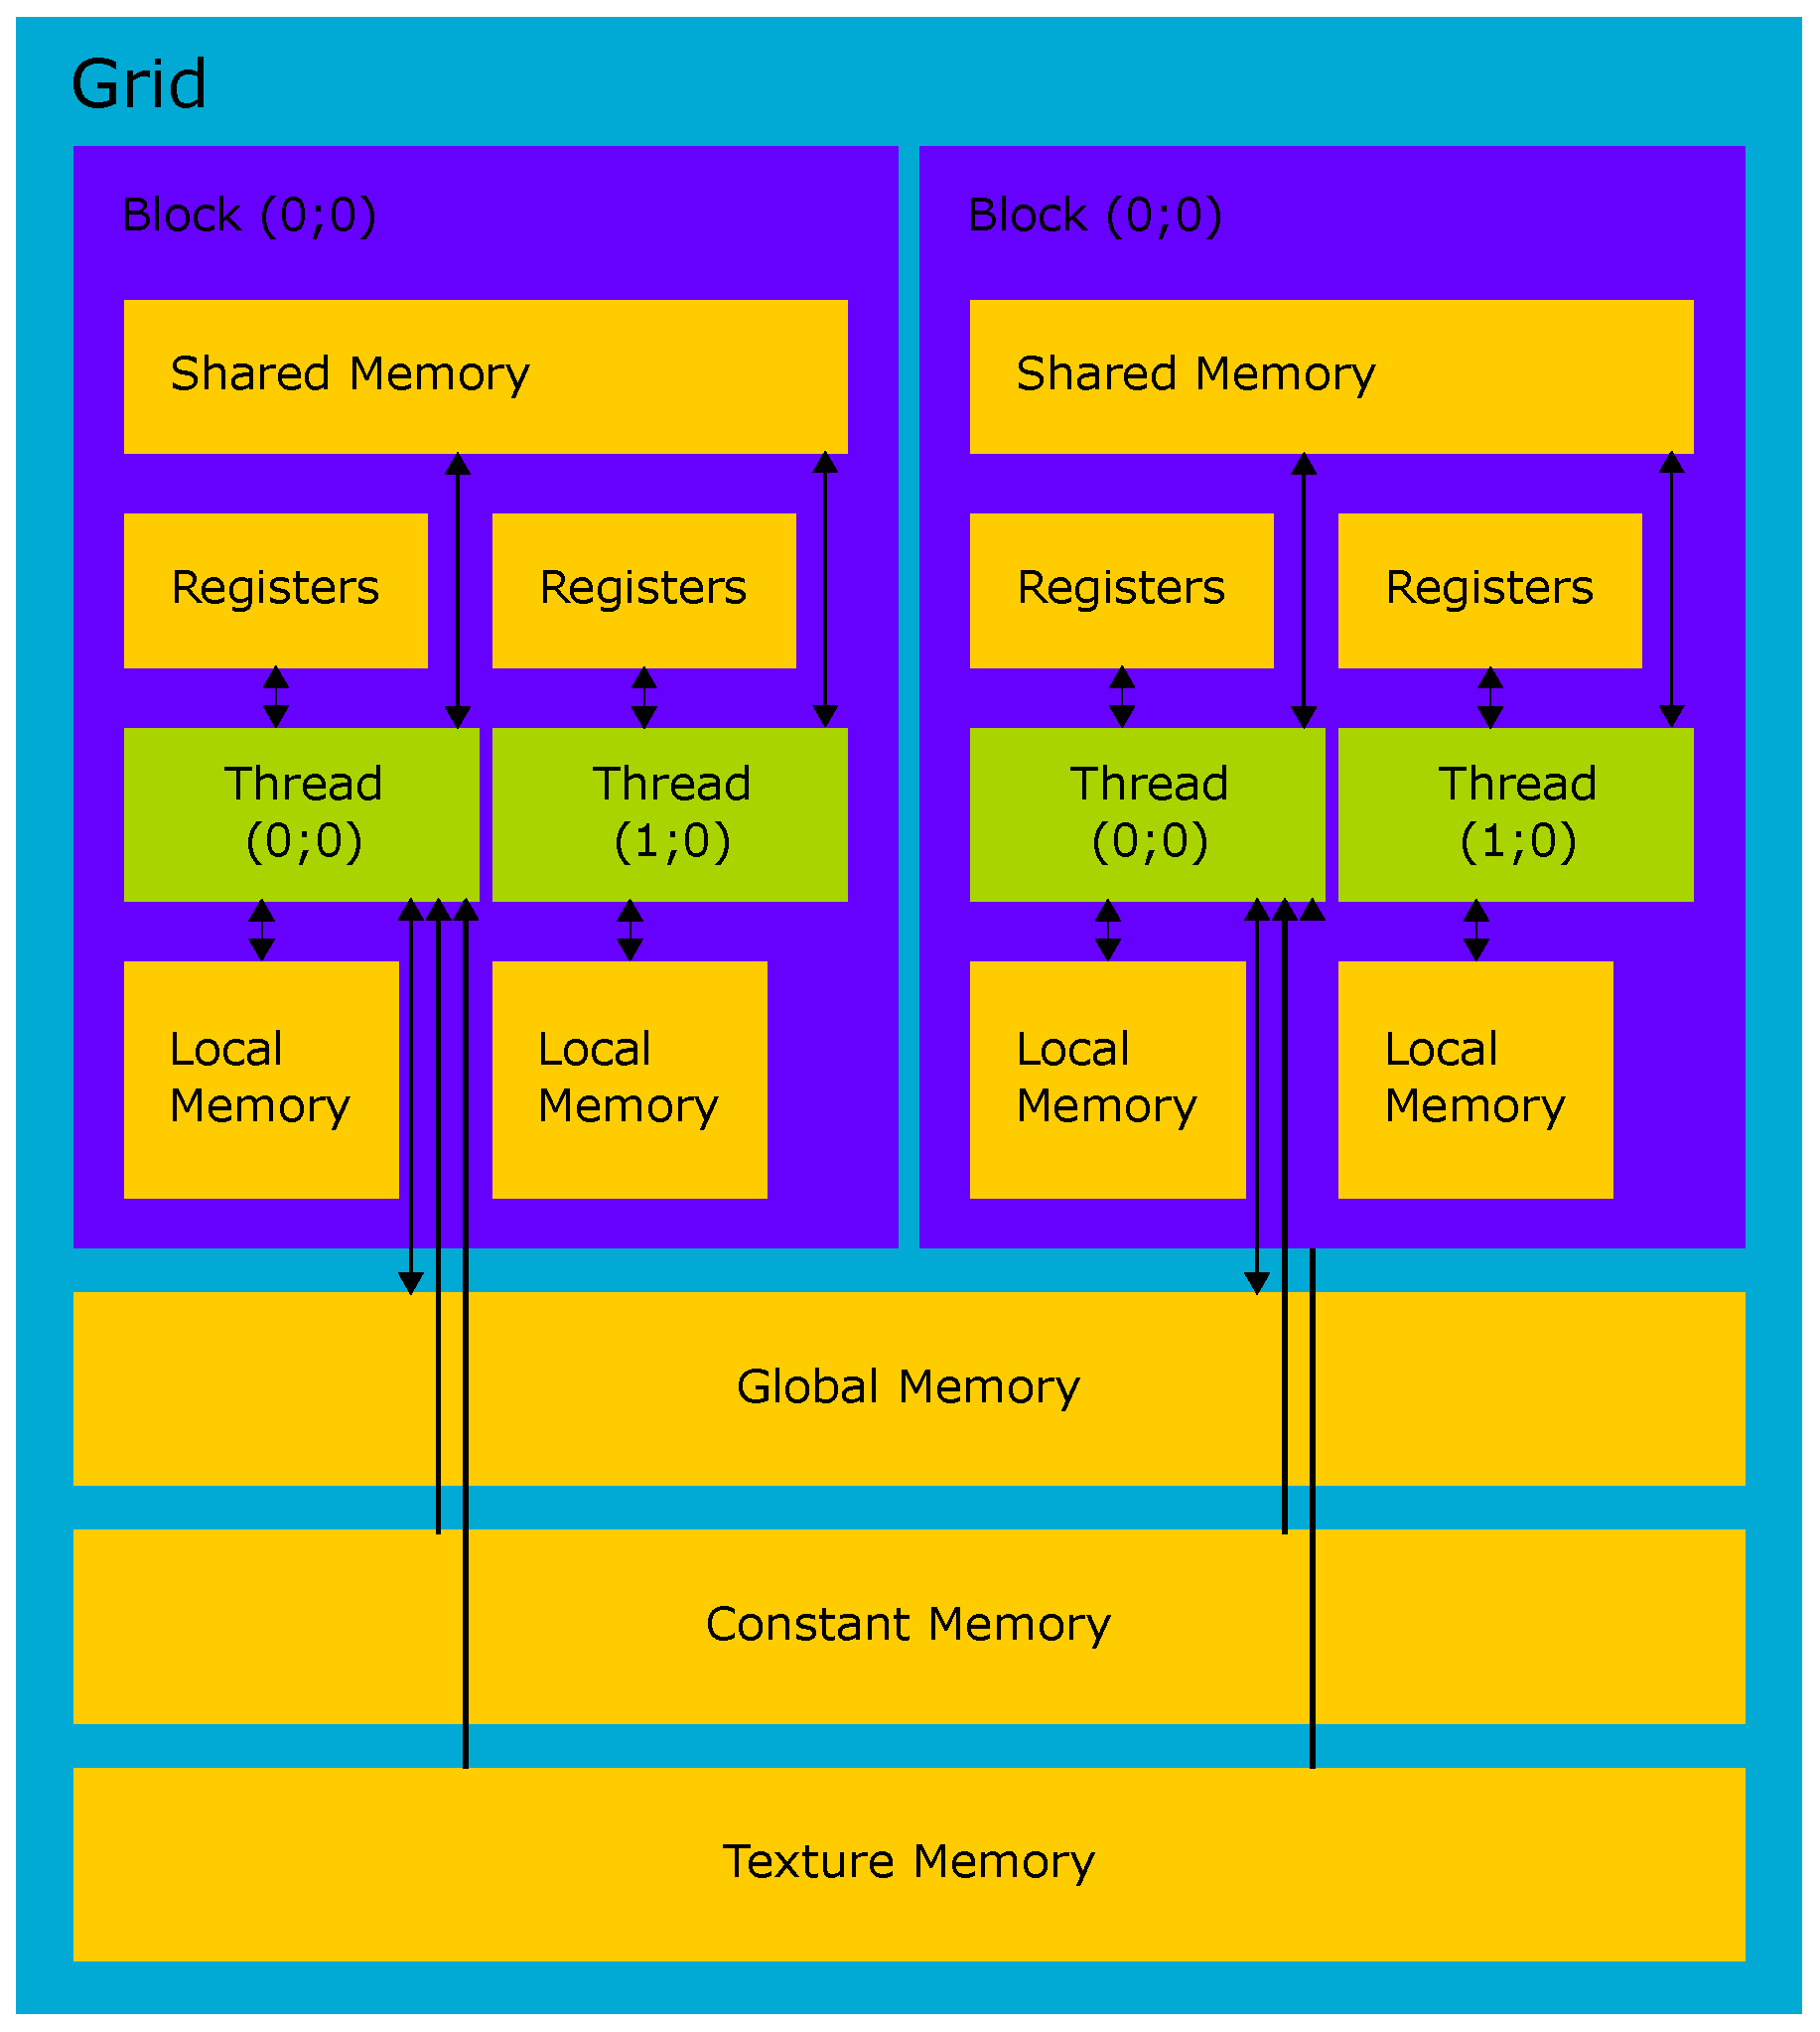
\includegraphics[width=0.6\linewidth]{img/CUDAmemAccess.eps}
  \caption{CUDA Memory access}
  \label{fig:cudamemaccess}
\end{figure}

\begin{description}
\item[Global memory] it is the largest memory (GBs) and it has high bandwidth (~100 GBps) but high latency (400-600 clock cycles). It is used for data storing data transfered from host memory and it is allocated and released in host code by special CUDA API function before kernel launch (Global memory allocation is independent on kernel, it could be used in many kernels without releasing and allocating new one for other kernel). Memory transfers are special host code CUDA API functions too, but they are asynchronous. Same as memory allocation/destroying, data are persistent between one kernel end end second kernel start. When data from this memory are processed, they are cached in L2 cache. Also processed data or output is stored here before it is transfered back to host. It is operated in transactions of 32B - 128B so for better performance it is better to access data aligned on transaction size. Physically, it is off the chip, but on the device.
\item[Shared memory] is memory is shared by all threads running on same SM. It has lower latency (32 bits / 2 cycles on CC 1.x and 2.x and 64 bits / 1 cycle on 3.x) than Global memory, but it is also smaller (depend on Compute Capability, from 16 kB on 1.x CC to 48kB on 2.x CC and 3.x CC). Memory is allocated on kernel launch (it is one of kernel function parameters) and data are copied from global memory in kernel run. Releasing of memory is done automatically after kernel is finished, so data stored here are not persistent between two kernels, they are even no persistent between same kernel runs.\\
This memory is divided into banks, each bank could be accessed independently which is really fast but if there are conflicts in accessing to same bank from multiple threads, access to the bank is serialized (except reading same address which is called broadcast) and could be many times slower, so for the best performance, it is better to avoid these conflicts (for example when threads accessing banks linearly~\ref{fig:linearaccess} or with stride~\ref{fig:strideaccess}, which is not a divisor of total banks count). On CC 1.x and CC 2.x, bank size is 32 bits, on CC 3.0 we can select between 32 bits and 64 bit banks. Physically it is situated near each processor for fast access.
\end{description}

\begin{figure}[h]
\centering
\begin{subfigure}{1.0\textwidth}
  \centering
  \includegraphics[width=.9\linewidth]{img/sharedMemoryLinearAccess.eps}
  \caption{Linear Access to shared memory}
  \label{fig:linearaccess}
\end{subfigure}
\begin{subfigure}{1.0\textwidth}
  \centering
  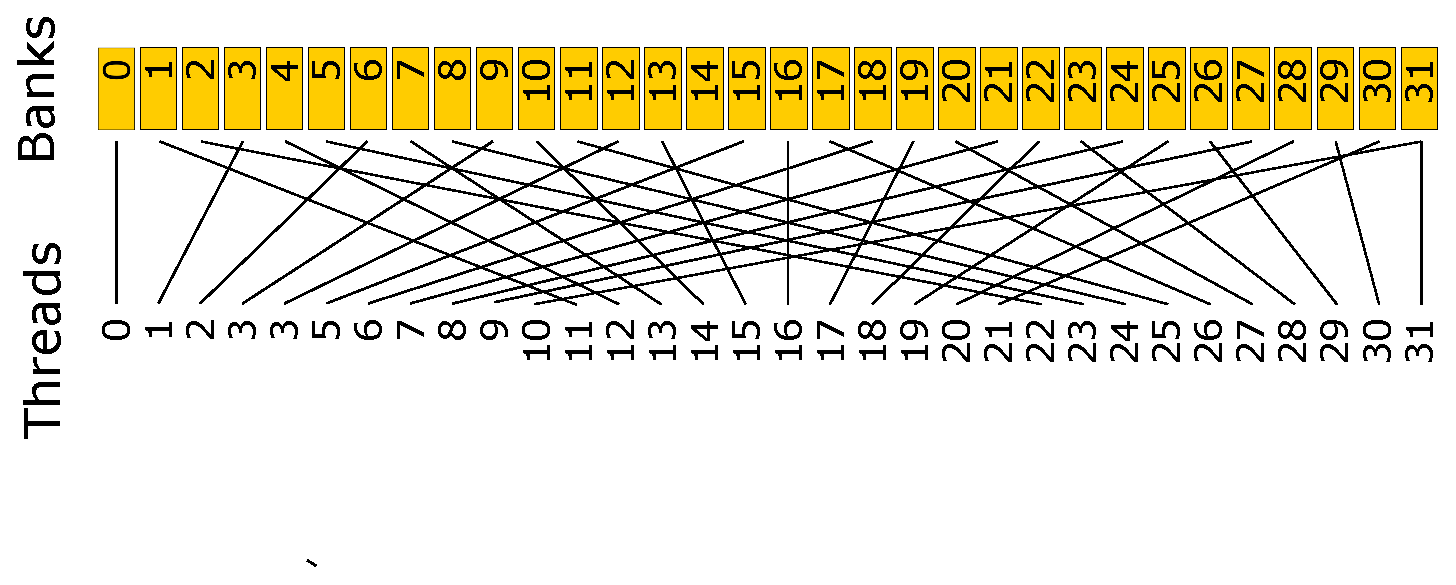
\includegraphics[width=.9\linewidth]{img/sharedMemoryStrideAccess.eps}
  \caption{Access to Shared Memory with stride 3}
  \label{fig:strideaccess}
\end{subfigure}
\caption{Shared Memory access}
\end{figure}

\begin{description}
\item[L1 Cache] has on most devices similar parameters as Share memory, because it has same resource. We can configure which memory should be preferred and bigger by special CUDA API function from host code. On CC 3.0, L1 cache was merged with texture cache and is independent on shared memory (resources are not shared).
\item[Registers] Each multiprocessor has own register pool. Depend on CC, it has 8-64k of 32-bit registers. registers are the smallest memory, but also has the smallest latency (they are as fast as cores). For programmer, registers are not directly controllable. Only slow down is read-after write dependency which takes 24 clock cycles, but it could be hidden by enough of active warps.
\item[Local memory] is memory reserved in Global memory accessible by a single thread only. Bigger data like structures and arrays are stored here because they don't fit into registers. Because of smaller register size, some of registers are deferred in local memory.
\item[Constant memory] is a special memory for read-only data. Its size is 64kB and from CC 2.x, compiler stores here constant, thread-independent variables. From CC 2.0, compiler is forced to loading all constant, thread independent variables into this cache.
\item[Texture memory] is special memory used for graphics. Its main benefit is 2D spatial locality used mainly for textures.
\end{description}

Data transfer between host and device are much slower than on device memory transfers (16/32 GBps depend on PCI Express version, but could be slowed by host memory), which could make CUDA inefficient for small data and compute inexpensive tasks. Transfer call has great overhead so bulk transfers are preferred over individually transfers. Data are copied from host code to device global memory but host memory could be mapped to the host memory space and than data could be accessed directly from device code (but with same, bad latency). Data transfer could be hidden by overlapping data transfer with computing, because CUDA device is capable of computing and simultaneously perform two asynchronous data transfers.

% is little bit different, because programmer can split execution of instructions into different branches by conditions based on thread identification. In both models